\titledquestion{Run DFS and BFS}

\newcommand{\stack}[5]{
    \begin{minipage}{.13\linewidth}
        \begin{tikzpicture}[scale=0.5]
            \cell{#1}
            \cell{#2}
            \cell{#3}
            \cell{#4}
            \cell{#5}
        \end{tikzpicture}
    \end{minipage}
}

Answer the following questions for the tree shown below \textbf{according to  the definition specified in the lecture slides}.

Note: Form your answer in the following steps.
\begin{enumerate}[1.]
    \item Decide on an appropriate \textbf{data structure} to implement the traversal.
    \item \textbf{Popping a node} and \textbf{pushing a sequence of children} can be considered as one single step.
    \item When doing \textbf{Breadth First Traversal}, push children of a node into the data structure in \textbf{alphabetical order}; when doing \textbf{Depth First Traversal}, push children of a node into the data structure in \textbf{reverse alphabetical order}.
\end{enumerate}
\textbf{Example: }
Given a tree with root \textbf{A}: \\
\begin{figure}[h]
    \centering
    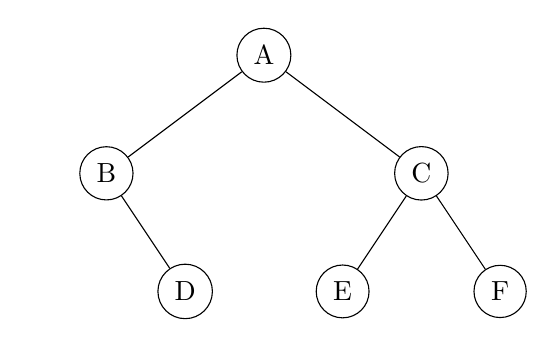
\begin{tikzpicture}[level distance=1.5cm,
        level 1/.style={sibling distance=4cm},
        level 2/.style={sibling distance=2cm},
        every node/.style = {draw, circle}]
        \node {A}
        child { node {B}
            child { edge from parent[draw=none] }
            child { node {D} }
        }
        child { node {C} 
            child { node {E}}
            child { node {F}}
        };
    \end{tikzpicture}
    \label{fig:example_pic}
\end{figure}

The process of doing \textbf{Breadth First Traversal} is: 

\begin{figure}[h]
    \centering
    \raisebox{-2.5em}{\text{front}} \raisebox{-2.5em}{$\rightarrow$}
    \stack{}{}{}{}{A} $\to$
    \stack{}{}{}{C}{B} $\to$
    \stack{}{}{}{D}{C} $\to$
    \stack{}{}{F}{E}{D} $\to$
    \stack{}{}{}{E}{F} $\to$
    \stack{}{}{}{}{F} $\to$
    \stack{}{}{}{}{}
    
    \label{fig:example_sol}
\end{figure}

\pagebreak
\begin{parts}
\part[5] Run \textbf{Pre-order Depth First Traversal} on the tree with root \textbf{A} and draw the whole process in the space below. (Note: it's not required to use all the blank cells.)
\begin{figure}[h]
    \centering 
    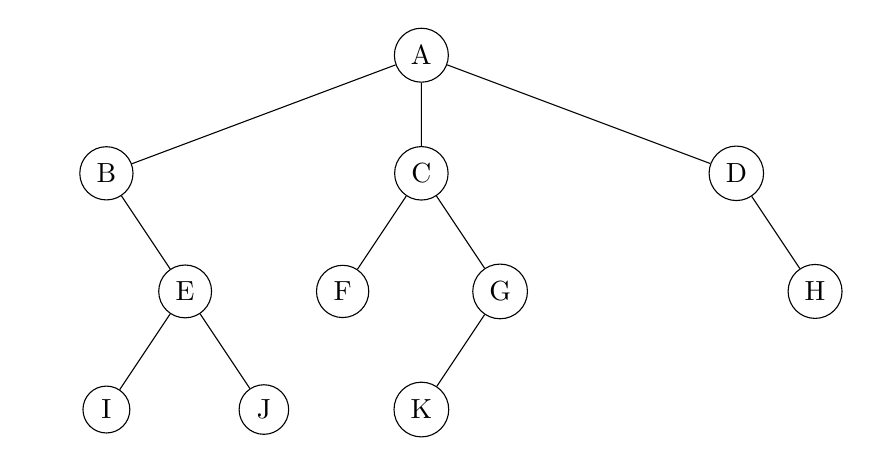
\begin{tikzpicture}[level distance=1.5cm,
        level 1/.style={sibling distance=4cm},
        level 2/.style={sibling distance=2cm},
        level 3/.style={sibling distance=2cm},
        level 4/.style={sibling distance=2cm},
        every node/.style = {draw, circle}]
        \node {A}
        child { node {B}
            child { edge from parent[draw=none] }
            child { node {E} 
                child { node {I} }
                child { node {J} }
            }
        }
        child { node {C} 
            child { node {F}
            }
            child { node {G}
                child { node {K} }
                child { edge from parent[draw=none] }
            }
        }
        child { node {D}
            child { edge from parent[draw=none] }
            child { node {H} }
        };
    \end{tikzpicture}
    \label{fig:example_pic}
\end{figure}
\begin{solution}\\\\
    \begin{minipage}{.14\linewidth}
            \begin{tikzpicture}[scale=0.5]
                \cell{}
                \cell{}
                \cell{}
                \cell{}
                \cell{}
            \end{tikzpicture}
        \end{minipage}
        $\to$
        \begin{minipage}{.14\linewidth}
            \begin{tikzpicture}[scale=0.5]
                \cell{}
                \cell{}
                \cell{}
                \cell{}
                \cell{}
            \end{tikzpicture}
        \end{minipage}
        $\to$
        \begin{minipage}{.14\linewidth}
            \begin{tikzpicture}[scale=0.5]
                \cell{}
                \cell{}
                \cell{}
                \cell{}
                \cell{}
            \end{tikzpicture}
        \end{minipage}
        $\to$
        \begin{minipage}{.14\linewidth}
            \begin{tikzpicture}[scale=0.5]
                \cell{}
                \cell{}
                \cell{}
                \cell{}
                \cell{}
            \end{tikzpicture}
        \end{minipage}
        $\to$
        \begin{minipage}{.14\linewidth}
            \begin{tikzpicture}[scale=0.5]
                \cell{}
                \cell{}
                \cell{}
                \cell{}
                \cell{}
            \end{tikzpicture}
        \end{minipage}
        $\to$

        \begin{minipage}{.14\linewidth}
            \begin{tikzpicture}[scale=0.5]
                \cell{}
                \cell{}
                \cell{}
                \cell{}
                \cell{}
            \end{tikzpicture}
        \end{minipage}
        $\to$
        \begin{minipage}{.14\linewidth}
            \begin{tikzpicture}[scale=0.5]
                \cell{}
                \cell{}
                \cell{}
                \cell{}
                \cell{}
            \end{tikzpicture}
        \end{minipage}
        $\to$
        \begin{minipage}{.14\linewidth}
            \begin{tikzpicture}[scale=0.5]
                \cell{}
                \cell{}
                \cell{}
                \cell{}
                \cell{}
            \end{tikzpicture}
        \end{minipage}
        $\to$
        \begin{minipage}{.14\linewidth}
            \begin{tikzpicture}[scale=0.5]
                \cell{}
                \cell{}
                \cell{}
                \cell{}
                \cell{}
            \end{tikzpicture}
        \end{minipage}
        $\to$
        \begin{minipage}{.14\linewidth}
            \begin{tikzpicture}[scale=0.5]
                \cell{}
                \cell{}
                \cell{}
                \cell{} 
                \cell{}
            \end{tikzpicture}
        \end{minipage}
        $\to$

        \begin{minipage}{.14\linewidth}
            \begin{tikzpicture}[scale=0.5]
                \cell{}
                \cell{}
                \cell{}
                \cell{}
                \cell{}
            \end{tikzpicture}
        \end{minipage}
        $\to$
        \begin{minipage}{.14\linewidth}
            \begin{tikzpicture}[scale=0.5]
                \cell{}
                \cell{}
                \cell{}
                \cell{}
                \cell{}
            \end{tikzpicture}
        \end{minipage}
        $\to$
        \begin{minipage}{.14\linewidth}
            \begin{tikzpicture}[scale=0.5]
                \cell{}
                \cell{}
                \cell{}
                \cell{}
                \cell{}
            \end{tikzpicture}
        \end{minipage}
        $\to$
        \begin{minipage}{.14\linewidth}
            \begin{tikzpicture}[scale=0.5]
                \cell{}
                \cell{}
                \cell{}
                \cell{}
                \cell{}
            \end{tikzpicture}
        \end{minipage}
        $\to$
        \begin{minipage}{.14\linewidth}
            \begin{tikzpicture}[scale=0.5]
                \cell{}
                \cell{}
                \cell{}
                \cell{}
                \cell{}
            \end{tikzpicture}
        \end{minipage}

\end{solution}

\pagebreak
    \part[5]  Run \textbf{Breadth First Traversal} on the tree with root \textbf{A} and draw the whole process in the space below. (Note: it's not required to use all the blank cells.)
    \begin{figure}[h]
    \centering
    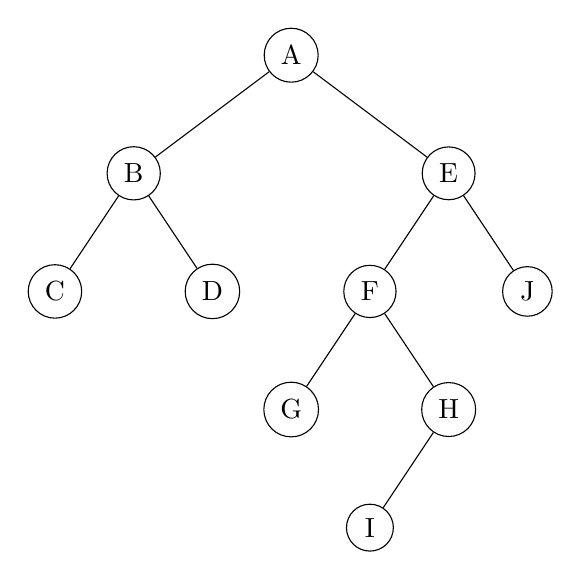
\begin{tikzpicture}[level distance=1.5cm,
        level 1/.style={sibling distance=4cm},
        level 2/.style={sibling distance=2cm},
        level 3/.style={sibling distance=2cm},
        every node/.style = {draw, circle}]
        \node {A}
        child { node {B}
            child { node {C} }
            child { node {D} }
        }
        child { node {E} 
            child { node {F}
                child { node {G}}
                child { node {H}
                    child {node {I}}
                    child { edge from parent[draw=none] }
                }
            }
            child { node {J}}
        };
    \end{tikzpicture}
    \label{fig:example_pic}
\end{figure}
\begin{solution}
\\\\
    \begin{minipage}{.14\linewidth}
            \begin{tikzpicture}[scale=0.5]
                \cell{}
                \cell{}
                \cell{}
                \cell{}
                \cell{}
            \end{tikzpicture}
        \end{minipage}
        $\to$
        \begin{minipage}{.14\linewidth}
            \begin{tikzpicture}[scale=0.5]
                \cell{}
                \cell{}
                \cell{}
                \cell{}
                \cell{}
            \end{tikzpicture}
        \end{minipage}
        $\to$
        \begin{minipage}{.14\linewidth}
            \begin{tikzpicture}[scale=0.5]
                \cell{}
                \cell{}
                \cell{}
                \cell{}
                \cell{}
            \end{tikzpicture}
        \end{minipage}
        $\to$
        \begin{minipage}{.14\linewidth}
            \begin{tikzpicture}[scale=0.5]
                \cell{}
                \cell{}
                \cell{}
                \cell{}
                \cell{}
            \end{tikzpicture}
        \end{minipage}
        $\to$
        \begin{minipage}{.14\linewidth}
            \begin{tikzpicture}[scale=0.5]
                \cell{}
                \cell{}
                \cell{}
                \cell{}
                \cell{}
            \end{tikzpicture}
        \end{minipage}
        $\to$

        \begin{minipage}{.14\linewidth}
            \begin{tikzpicture}[scale=0.5]
                \cell{}
                \cell{}
                \cell{}
                \cell{}
                \cell{}
            \end{tikzpicture}
        \end{minipage}
        $\to$
        \begin{minipage}{.14\linewidth}
            \begin{tikzpicture}[scale=0.5]
                \cell{}
                \cell{}
                \cell{}
                \cell{}
                \cell{}
            \end{tikzpicture}
        \end{minipage}
        $\to$
        \begin{minipage}{.14\linewidth}
            \begin{tikzpicture}[scale=0.5]
                \cell{}
                \cell{}
                \cell{}
                \cell{}
                \cell{}
            \end{tikzpicture}
        \end{minipage}
        $\to$
        \begin{minipage}{.14\linewidth}
            \begin{tikzpicture}[scale=0.5]
                \cell{}
                \cell{}
                \cell{}
                \cell{}
                \cell{}
            \end{tikzpicture}
        \end{minipage}
        $\to$
        \begin{minipage}{.14\linewidth}
            \begin{tikzpicture}[scale=0.5]
                \cell{}
                \cell{}
                \cell{}
                \cell{} 
                \cell{}
            \end{tikzpicture}
        \end{minipage}
        $\to$

        \begin{minipage}{.14\linewidth}
            \begin{tikzpicture}[scale=0.5]
                \cell{}
                \cell{}
                \cell{}
                \cell{}
                \cell{}
            \end{tikzpicture}
        \end{minipage}
        $\to$
        \begin{minipage}{.14\linewidth}
            \begin{tikzpicture}[scale=0.5]
                \cell{}
                \cell{}
                \cell{}
                \cell{}
                \cell{}
            \end{tikzpicture}
        \end{minipage}
        $\to$
        \begin{minipage}{.14\linewidth}
            \begin{tikzpicture}[scale=0.5]
                \cell{}
                \cell{}
                \cell{}
                \cell{}
                \cell{}
            \end{tikzpicture}
        \end{minipage}
        $\to$
        \begin{minipage}{.14\linewidth}
            \begin{tikzpicture}[scale=0.5]
                \cell{}
                \cell{}
                \cell{}
                \cell{}
                \cell{}
            \end{tikzpicture}
        \end{minipage}
        $\to$
        \begin{minipage}{.14\linewidth}
            \begin{tikzpicture}[scale=0.5]
                \cell{}
                \cell{}
                \cell{}
                \cell{}
                \cell{}
            \end{tikzpicture}
        \end{minipage}

\end{solution}


\end{parts}